% Figura 2: Estrategias de optimización
\documentclass[border=5pt]{standalone}
\usepackage{tikz}
\usetikzlibrary{arrows.meta, decorations.pathreplacing, patterns}

\begin{document}

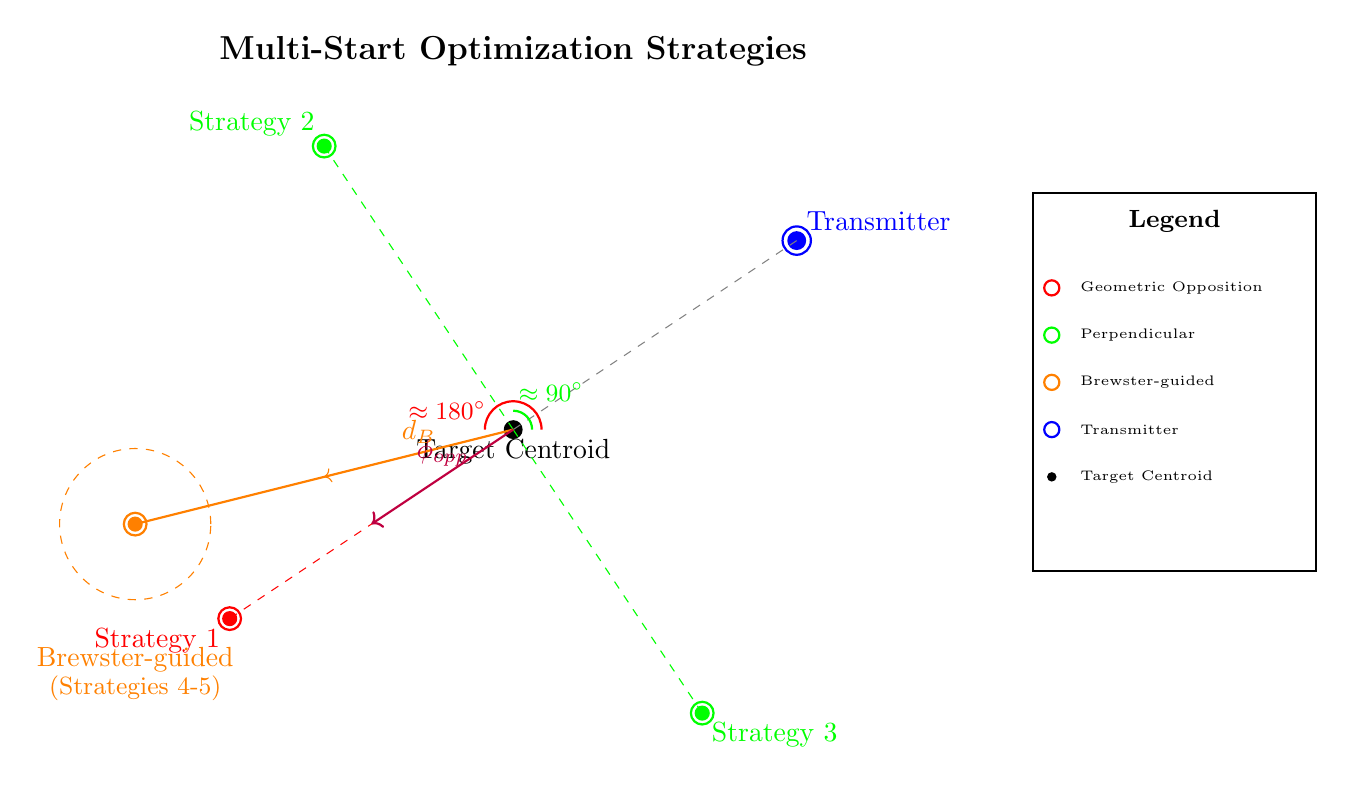
\begin{tikzpicture}[scale=1.2]

% Centro de targets
\coordinate (Center) at (0, 0);
\fill[black] (Center) circle (0.1);
\node[below] at (Center) {Target Centroid};

% Transmisor
\coordinate (Tx) at (3, 2);
\draw[blue, thick] (Tx) circle (0.15);
\fill[blue] (Tx) circle (0.1);
\node[above right, blue] at (Tx) {Transmitter};

% Línea Tx-Center
\draw[gray, dashed] (Tx) -- (Center);

% Estrategia 1: Posición opuesta
\coordinate (Rx1) at (-3, -2);
\draw[red, thick] (Rx1) circle (0.12);
\fill[red] (Rx1) circle (0.08);
\node[below left, red] at (Rx1) {Strategy 1};
\draw[red, dashed] (Center) -- (Rx1);

% Estrategia 2: Perpendicular
\coordinate (Rx2) at (-2, 3);
\draw[green, thick] (Rx2) circle (0.12);
\fill[green] (Rx2) circle (0.08);
\node[above left, green] at (Rx2) {Strategy 2};
\draw[green, dashed] (Center) -- (Rx2);

% Estrategia 3: Perpendicular opuesta
\coordinate (Rx3) at (2, -3);
\draw[green, thick] (Rx3) circle (0.12);
\fill[green] (Rx3) circle (0.08);
\node[below right, green] at (Rx3) {Strategy 3};
\draw[green, dashed] (Center) -- (Rx3);

% Estrategia 4-5: Brewster-guided (con zona de aleatoriedad)
\coordinate (RxBrewster) at (-4, -1);
\draw[orange, thick] (RxBrewster) circle (0.12);
\fill[orange] (RxBrewster) circle (0.08);

% Zona de aleatoriedad alrededor del punto Brewster
\draw[orange, dashed] (RxBrewster) circle (0.8);
\node[below, orange] at (-4, -2.2) {Brewster-guided};
\node[below, orange, font=\small] at (-4, -2.5) {(Strategies 4-5)};

% Ángulo de Brewster ilustrativo
\draw[orange, thick] (Center) -- (RxBrewster);
\draw[orange, ->] (Center) -- (-2, -0.5) node[midway, above] {$d_B$};

% Azimut opuesto
\draw[purple, thick, ->] (Center) -- (-1.5, -1) node[midway, above] {$\phi_{opp}$};

% Ángulo bistático para Strategy 1
\draw[red, thick] (Center) ++(0.3, 0) arc (0:180:0.3);
\node[red, font=\small] at (-0.7, 0.2) {$\approx 180^\circ$};

% Ángulos bistáticos para perpendiculares
\draw[green, thick] (Center) ++(0.2, 0) arc (0:90:0.2);
\node[green, font=\small] at (0.4, 0.4) {$\approx 90^\circ$};

% Etiquetas adicionales
\node[font=\large\bfseries] at (0, 4) {Multi-Start Optimization Strategies};

% Leyenda
\begin{scope}[shift={(5.5, 1)}]
    \draw[thick] (0, 1.5) rectangle (3, -2.5);
    \node[font=\small\bfseries] at (1.5, 1.2) {Legend};
    
    \draw[red, thick] (0.2, 0.5) circle (0.08);
    \node[font=\tiny, right] at (0.4, 0.5) {Geometric Opposition};
    
    \draw[green, thick] (0.2, 0) circle (0.08);
    \node[font=\tiny, right] at (0.4, 0) {Perpendicular};
    
    \draw[orange, thick] (0.2, -0.5) circle (0.08);
    \node[font=\tiny, right] at (0.4, -0.5) {Brewster-guided};
    
    \draw[blue, thick] (0.2, -1) circle (0.08);
    \node[font=\tiny, right] at (0.4, -1) {Transmitter};
    
    \fill[black] (0.2, -1.5) circle (0.05);
    \node[font=\tiny, right] at (0.4, -1.5) {Target Centroid};
\end{scope}

\end{tikzpicture}
\end{document}